\icode{E-MI-SI-L3-261104-001}
如图所示，光滑的四分之一圆弧轨道\(AD\)固定在竖直面内，圆弧的最低点D的切线方向水平，圆弧上的\(B\)、\(C\)两点将圆弧\(AD\)三等分。将一个小球放在\(B\)点，用一个最小的力\(F_1\)使小球静止在\(B\)点，再将小球移至\(C\)点，仍用最小的力\(F_2\)使小球静止在\(C\)点，则\(F_1:F_2\)等于\paren[]
	
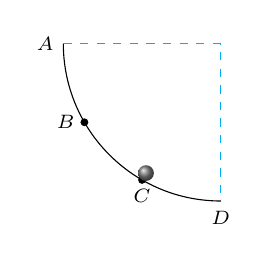
\begin{tikzpicture}[font=\scriptsize]
	\draw (-2,0)node[left]{\(A\)} arc(180:270:2)node[below]{\(D\)};
	\draw[dashed,cyan] (-2,0)--(0,0)--(0,-2);
	\fill (-150:2)node[left]{\(B\)} circle(.05) (-120:2)node[below]{\(C\)} circle(.05);
	\shade[ball color=gray] (-120:1.9) circle(.1);
\end{tikzpicture}
\begin{choices}
	\item \(1:\sqrt{3}\)
	\item \(\sqrt{3}:1\)
	\item \(1:3\)
	\item \(3:1\)
\end{choices}
\begin{answer}
	B\qquad 提示：当外力\(F\)与轨道对小球的支持力\(N\)垂直时，\(F\)最小
\end{answer}